\section{User Interface Wireframe}


\begin{figure}[H]
        \centering
        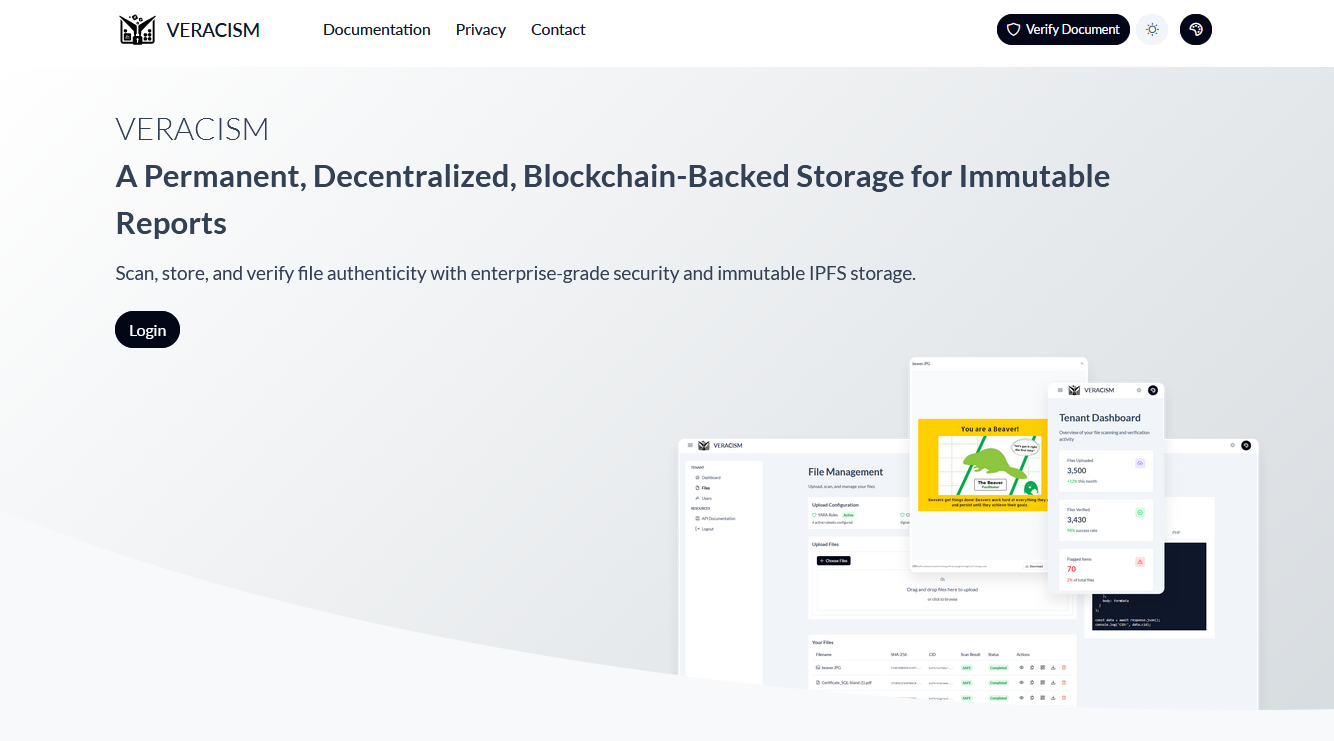
\includegraphics[height=0.35\textheight,keepaspectratio]{Texfiles/images/System Design/landing1.PNG}
        \caption{Landing Page - Hero Section}
        \label{fig:landing-page}
    \end{figure}

\begin{figure}[H]
        \centering
        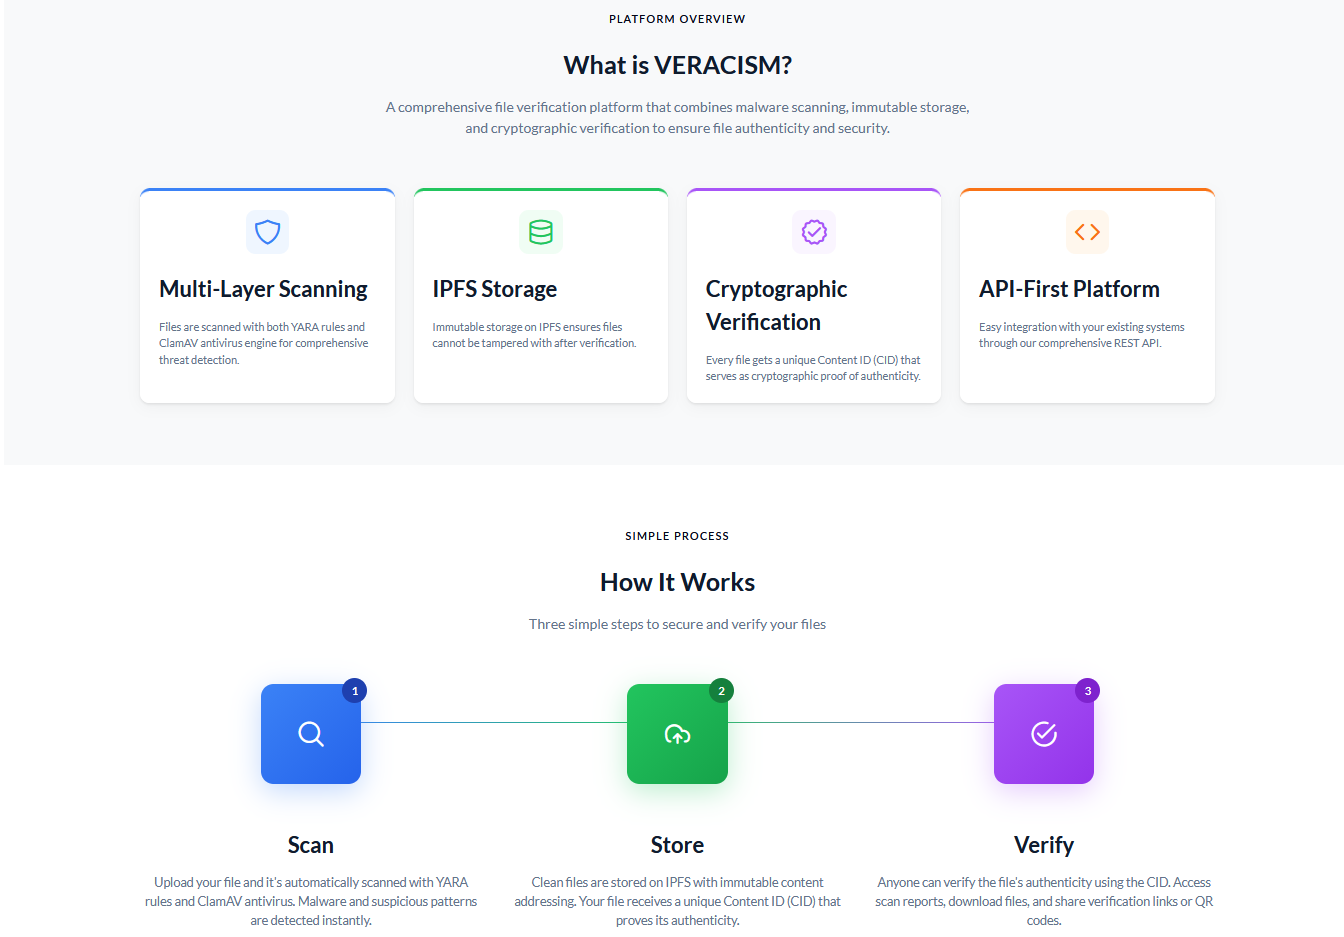
\includegraphics[height=0.37\textheight,keepaspectratio]{Texfiles/images/System Design/landing2.PNG}
        \caption{Landing Page - About / How It Works Section}
        \label{fig:landing-page-about}
\end{figure}

\begin{figure}[H]
        \centering
        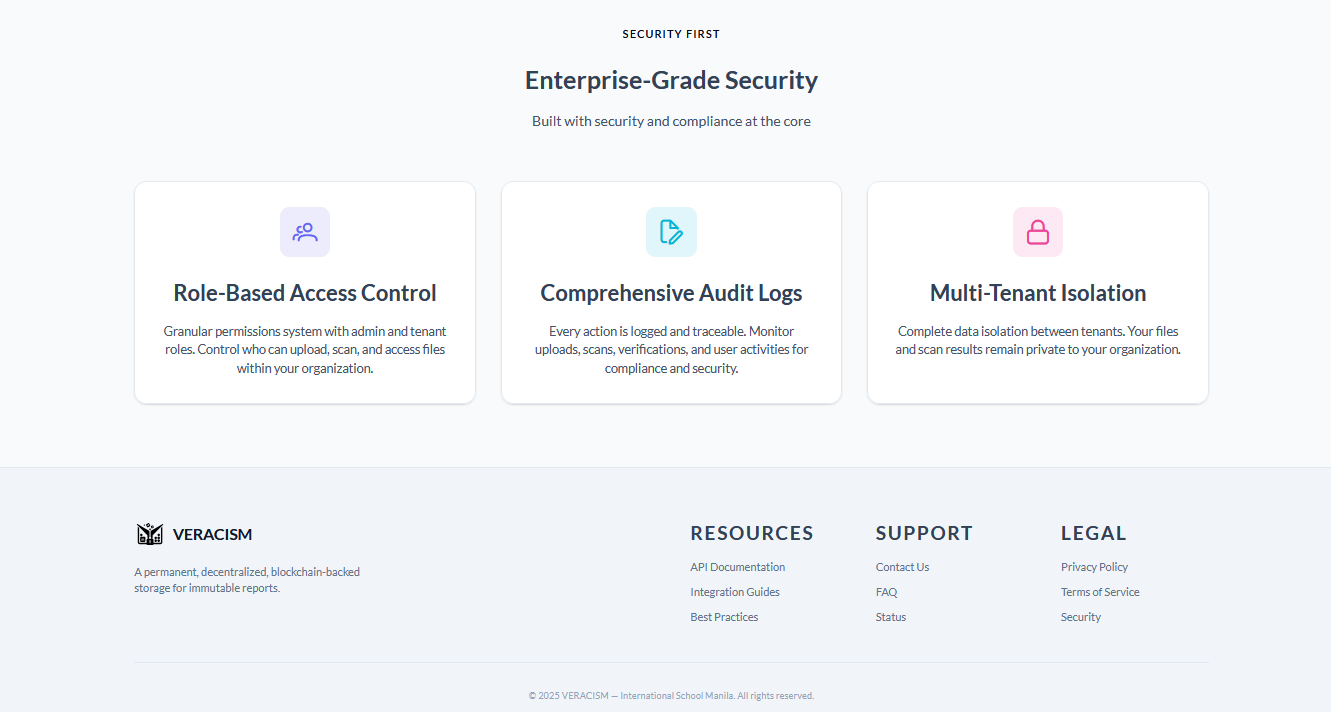
\includegraphics[height=0.32\textheight,keepaspectratio]{Texfiles/images/System Design/landing3.PNG}
        \caption{Landing Page - Footer Section}
        \label{fig:landing-page-footer}
\end{figure}

% Landing Page 

Landing page presents a permanent, decentralized, blockchain-backed file verification platform that scans, stores, and verifies documents using multi-layer malware scanning, IPFS immutable storage, and cryptographic verification. It highlights simple Scan-Store-Verify workflows, enterprise-grade security with role-based access, audit logs, multi-tenant isolation, and API-first integration.

\clearpage

\begin{figure}[H]
        \centering
        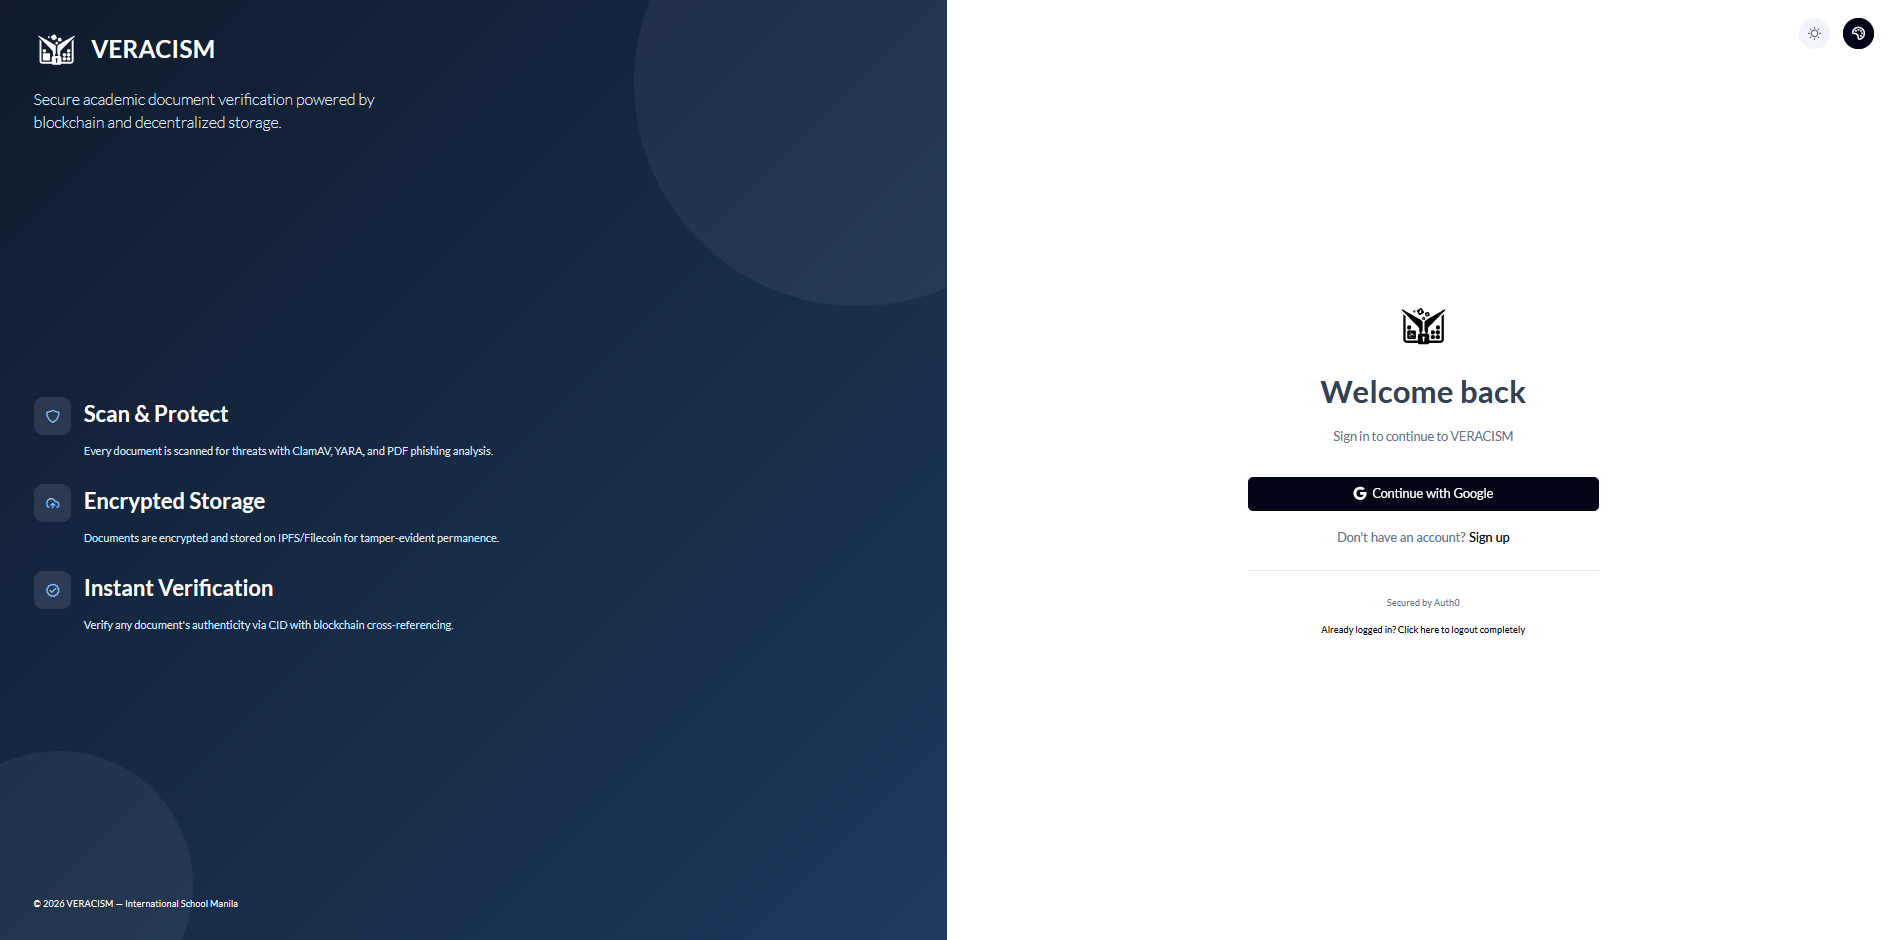
\includegraphics[height=0.35\textheight,keepaspectratio]{Texfiles/images/System Design/login.PNG}
        \caption{Login Page}
        \label{fig:landing-page}
    \end{figure}

\begin{figure}[H]
        \centering
        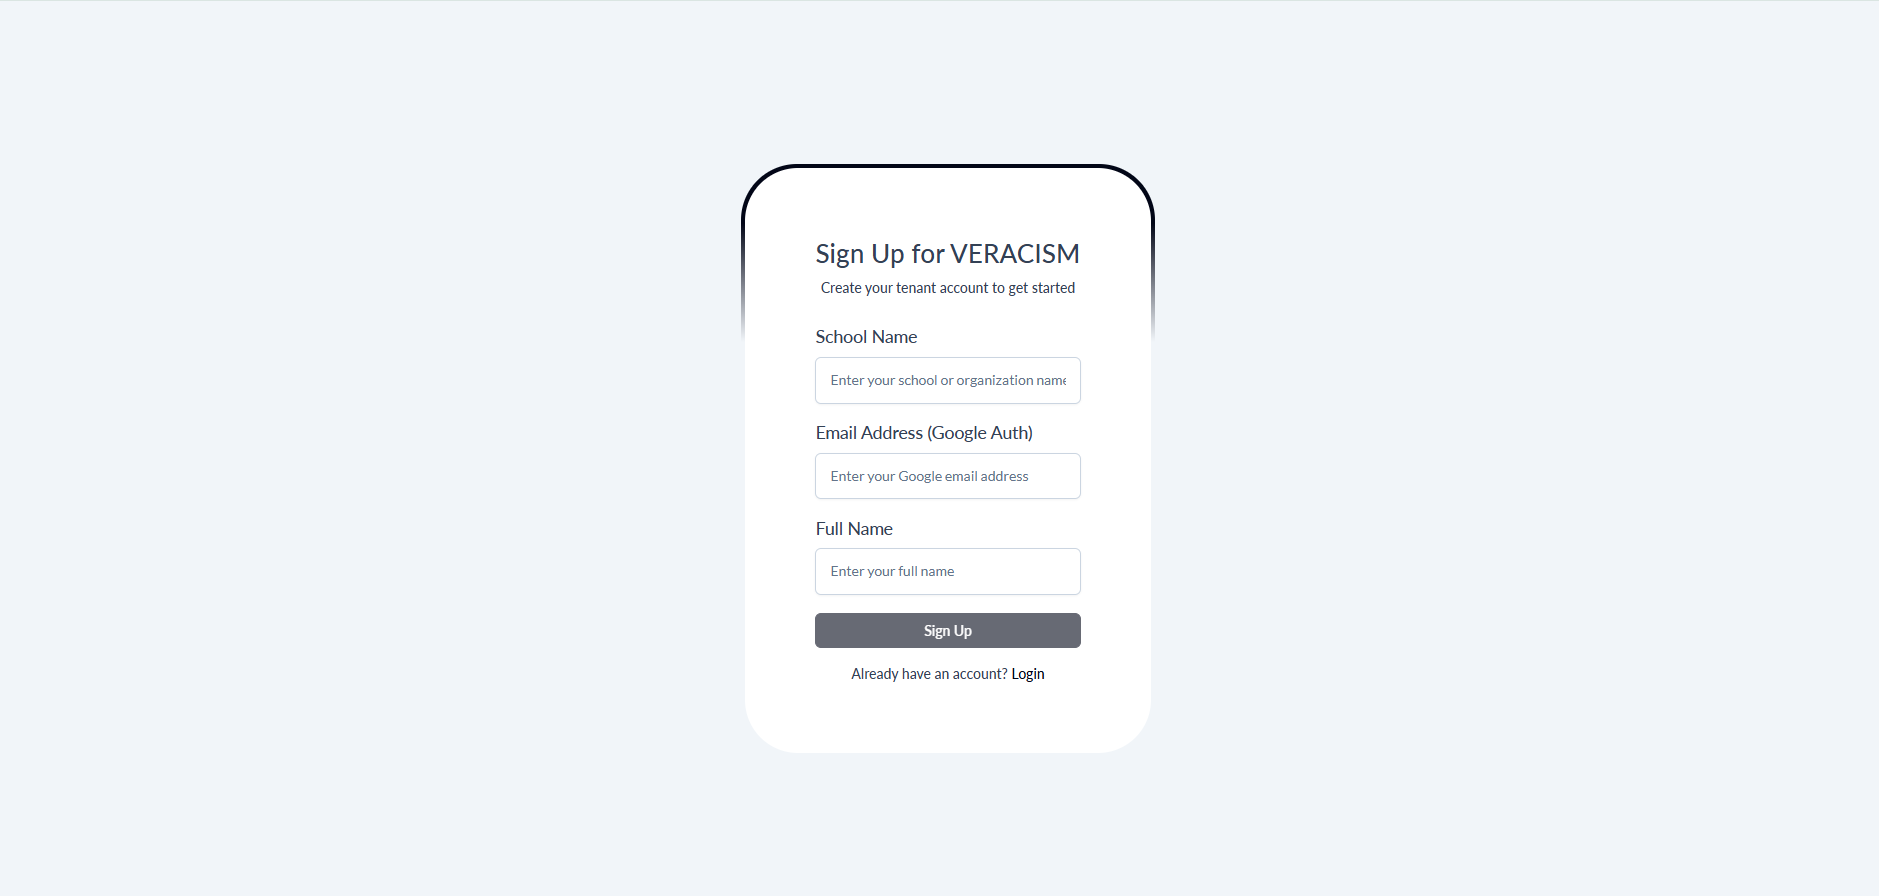
\includegraphics[height=0.35\textheight,keepaspectratio]{Texfiles/images/System Design/Signup.PNG}
        \caption{Sign up Page}
        \label{fig:signup-page}
\end{figure}

Veracism auth flow features a clean, centered card layout for both signup and login. New tenants can register by entering their school name, Google-based email, and full name, while existing users sign in using “Continue with Google,” managed by Auth0. After authentication, users are automatically routed to their own dashboard based on their role.

\clearpage

\begin{figure}[H]
        \centering
        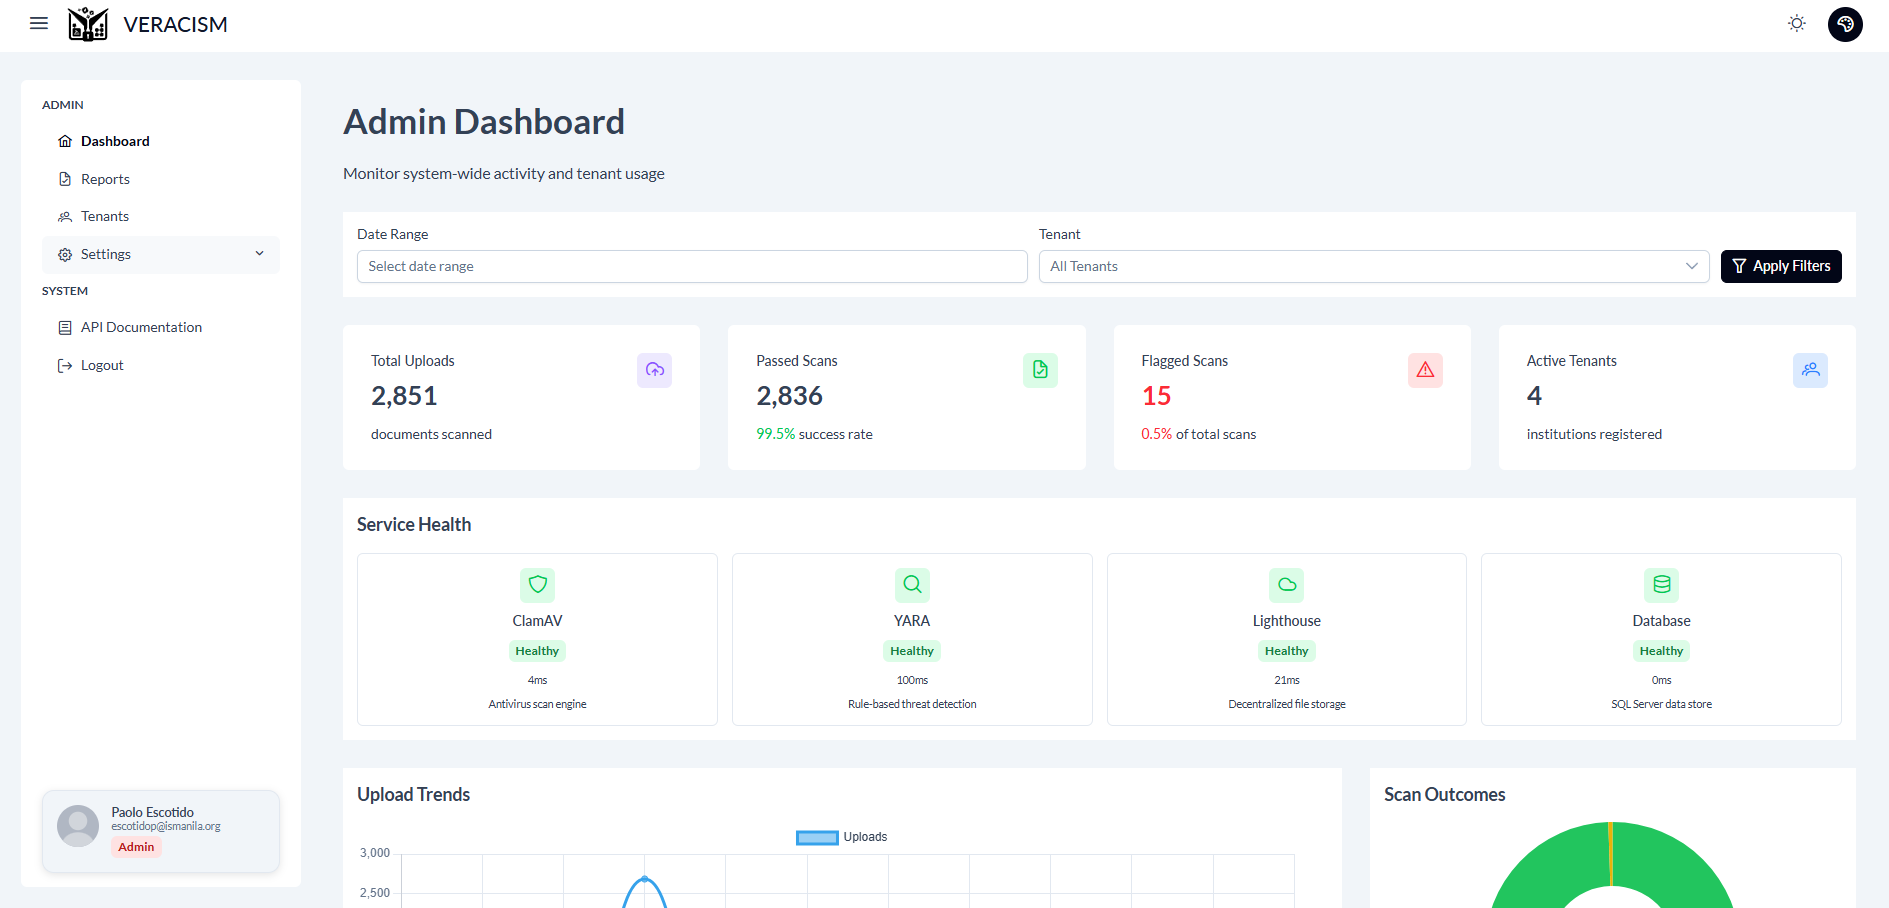
\includegraphics[height=0.35\textheight,keepaspectratio]{Texfiles/images/System Design/AdminDashboard.PNG}
        \caption{Admin - Dashboard Page}
        \label{fig:admin-dashboard}
    \end{figure}

    After an admin logs in, they see this analytics dashboard showing system-wide file uploads, scan results, active tenants, filters by date/tenant/type, and visual trends for uploads and scan outcomes.

\begin{figure}[H]
        \centering
        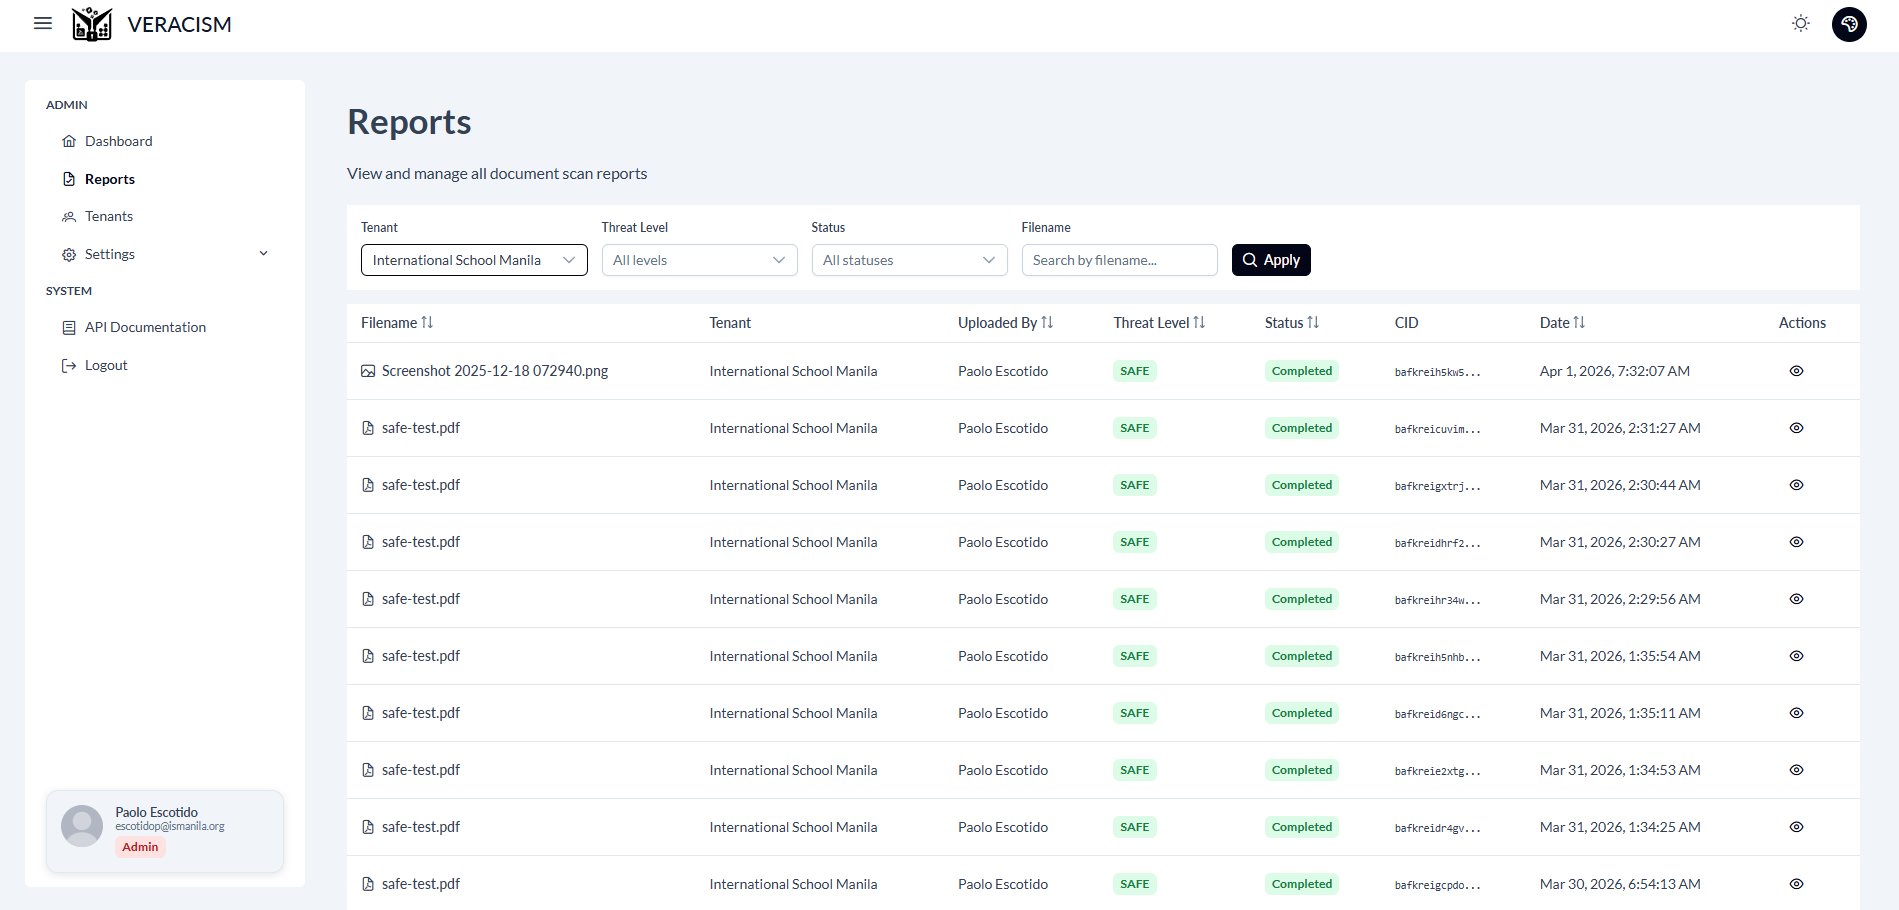
\includegraphics[height=0.35\textheight,keepaspectratio]{Texfiles/images/System Design/AdminReports.PNG}
        \caption{Admin - Reports}
        \label{fig:admin-reports}
\end{figure}

    Admin Reports page lets admins review the report uploaded in all registered tenant organizations.


\begin{figure}[H]
        \centering
        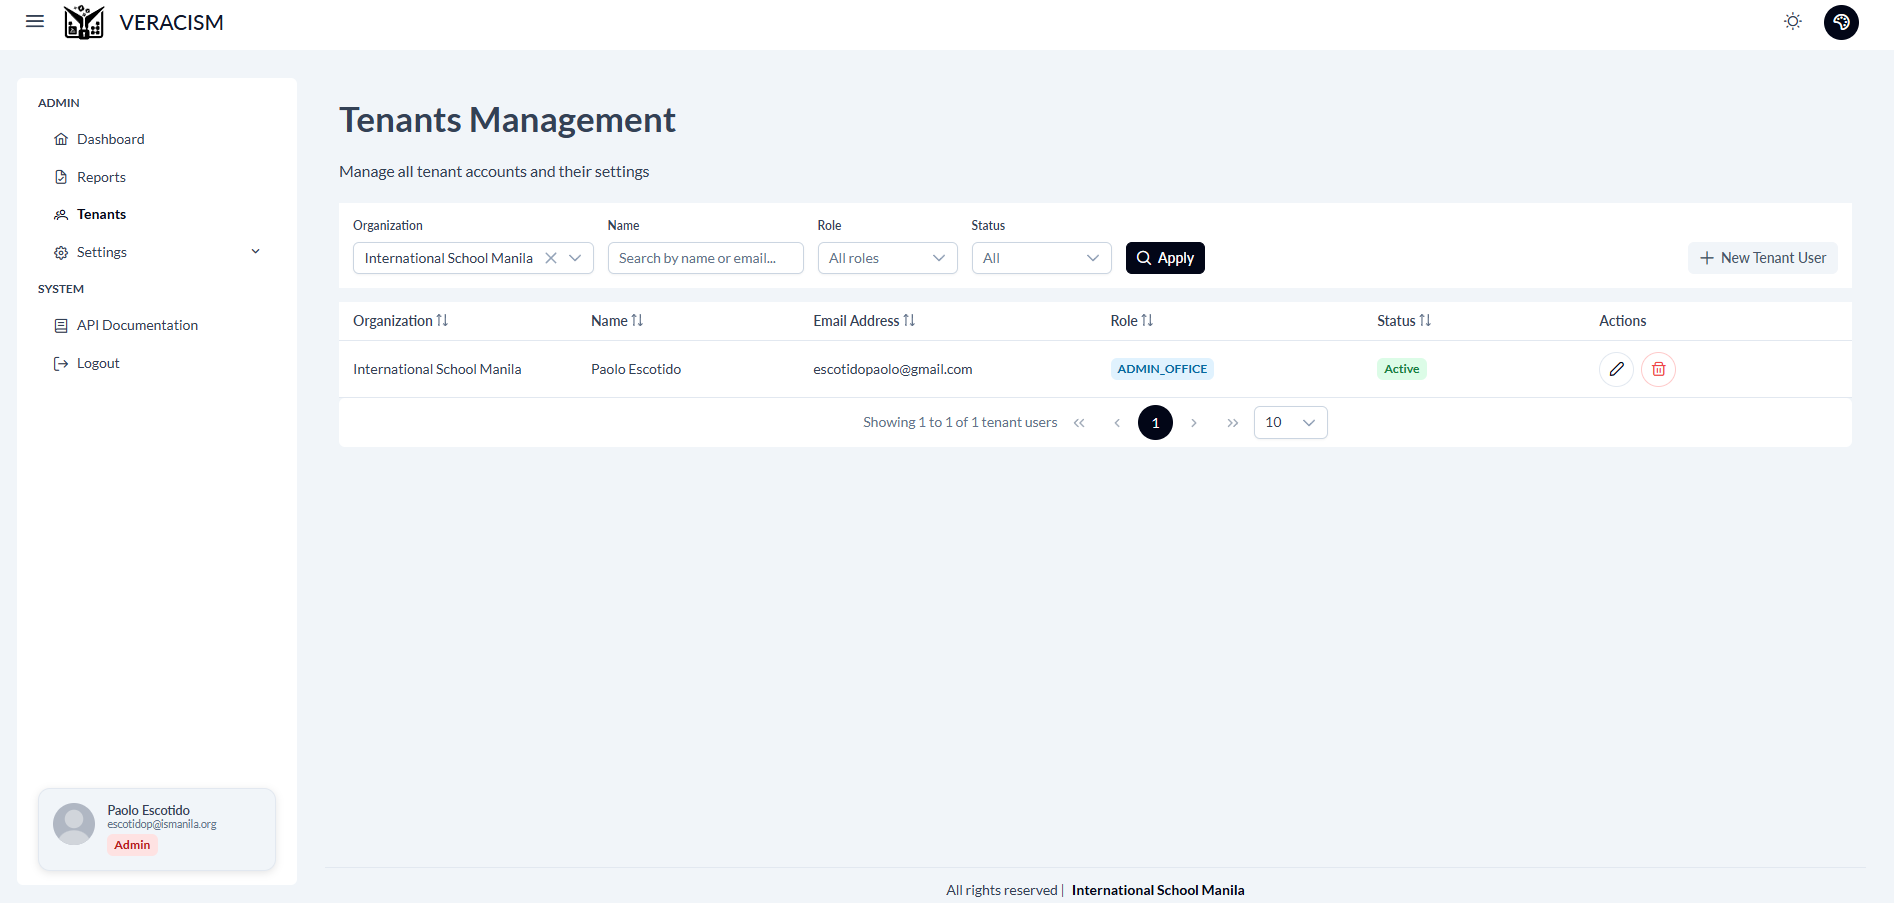
\includegraphics[height=0.35\textheight,keepaspectratio]{Texfiles/images/System Design/AdminTenants.PNG}
        \caption{Admin - Tenants Management}
        \label{fig:admin-tenants}
\end{figure}

    Admin Tenants page lets admins review, approve, and manage all registered tenant organizations, including their users, roles, status, and actions.

\begin{figure}[H]
        \centering
        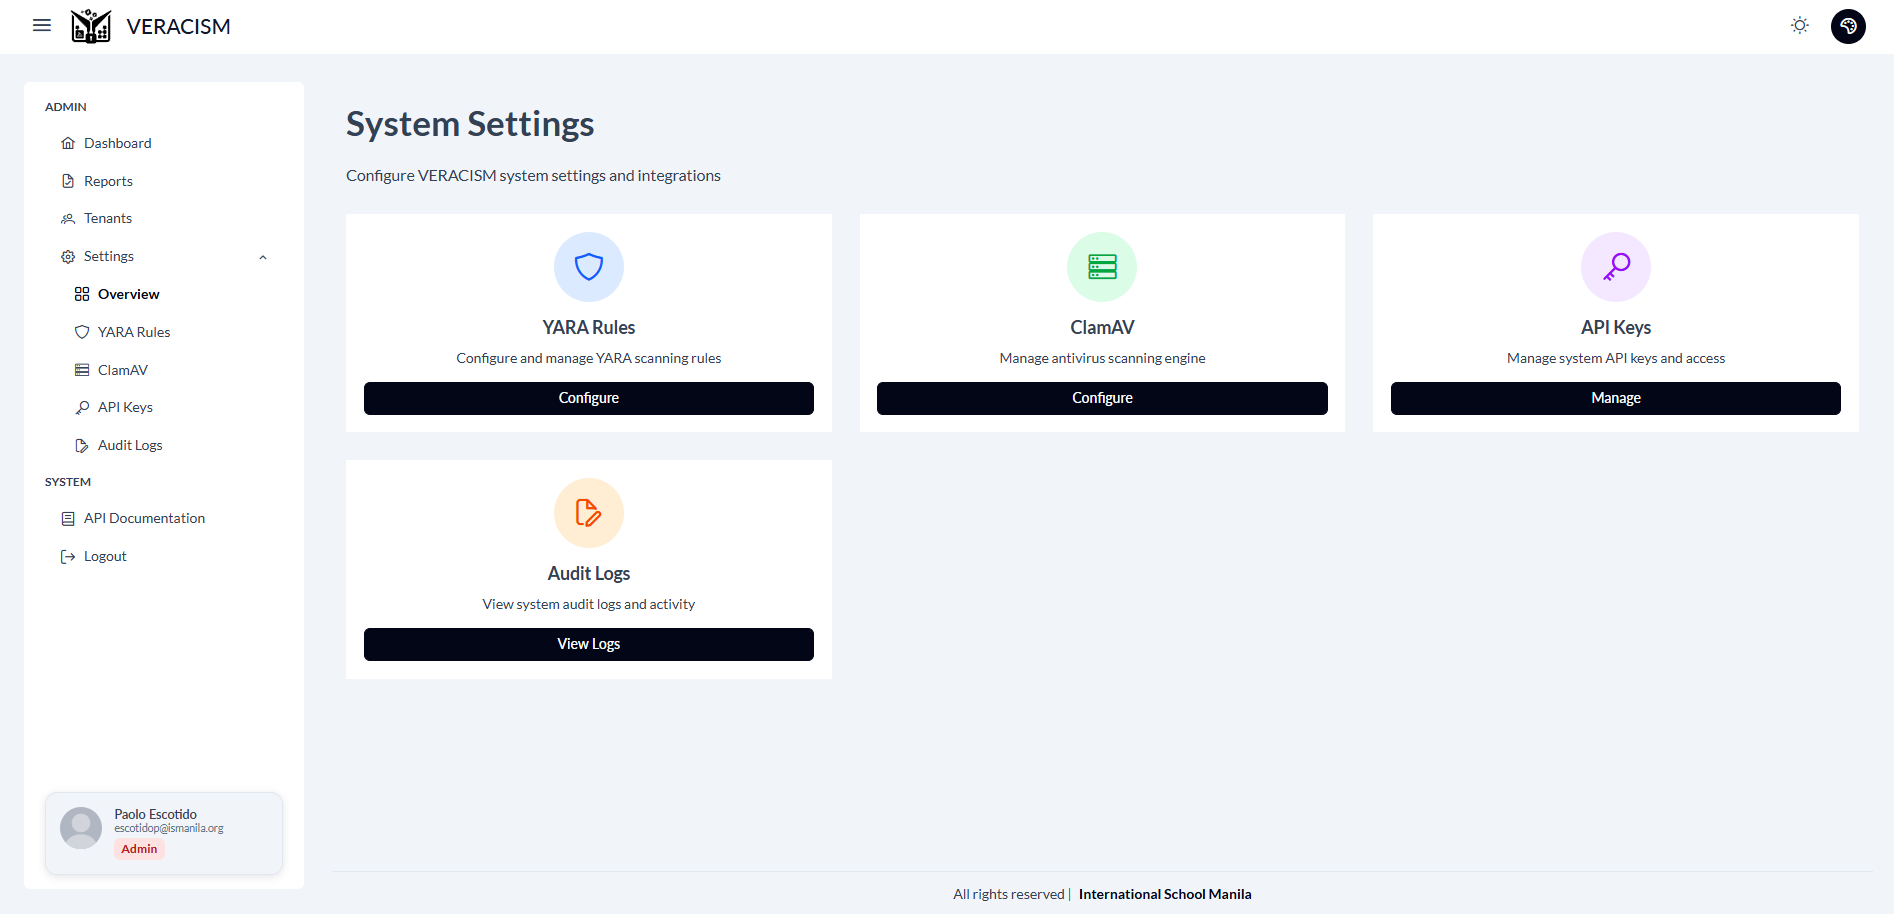
\includegraphics[height=0.35\textheight,keepaspectratio]{Texfiles/images/System Design/AdminSettings.PNG}
        \caption{Admin - Settings Page}
        \label{fig:admin-settings}
    \end{figure}

    System Settings page lets admins configure YARA rules, manage the ClamAV antivirus engine, control API keys, and review system audit logs for Veracism.

\begin{figure}[H]
        \centering
        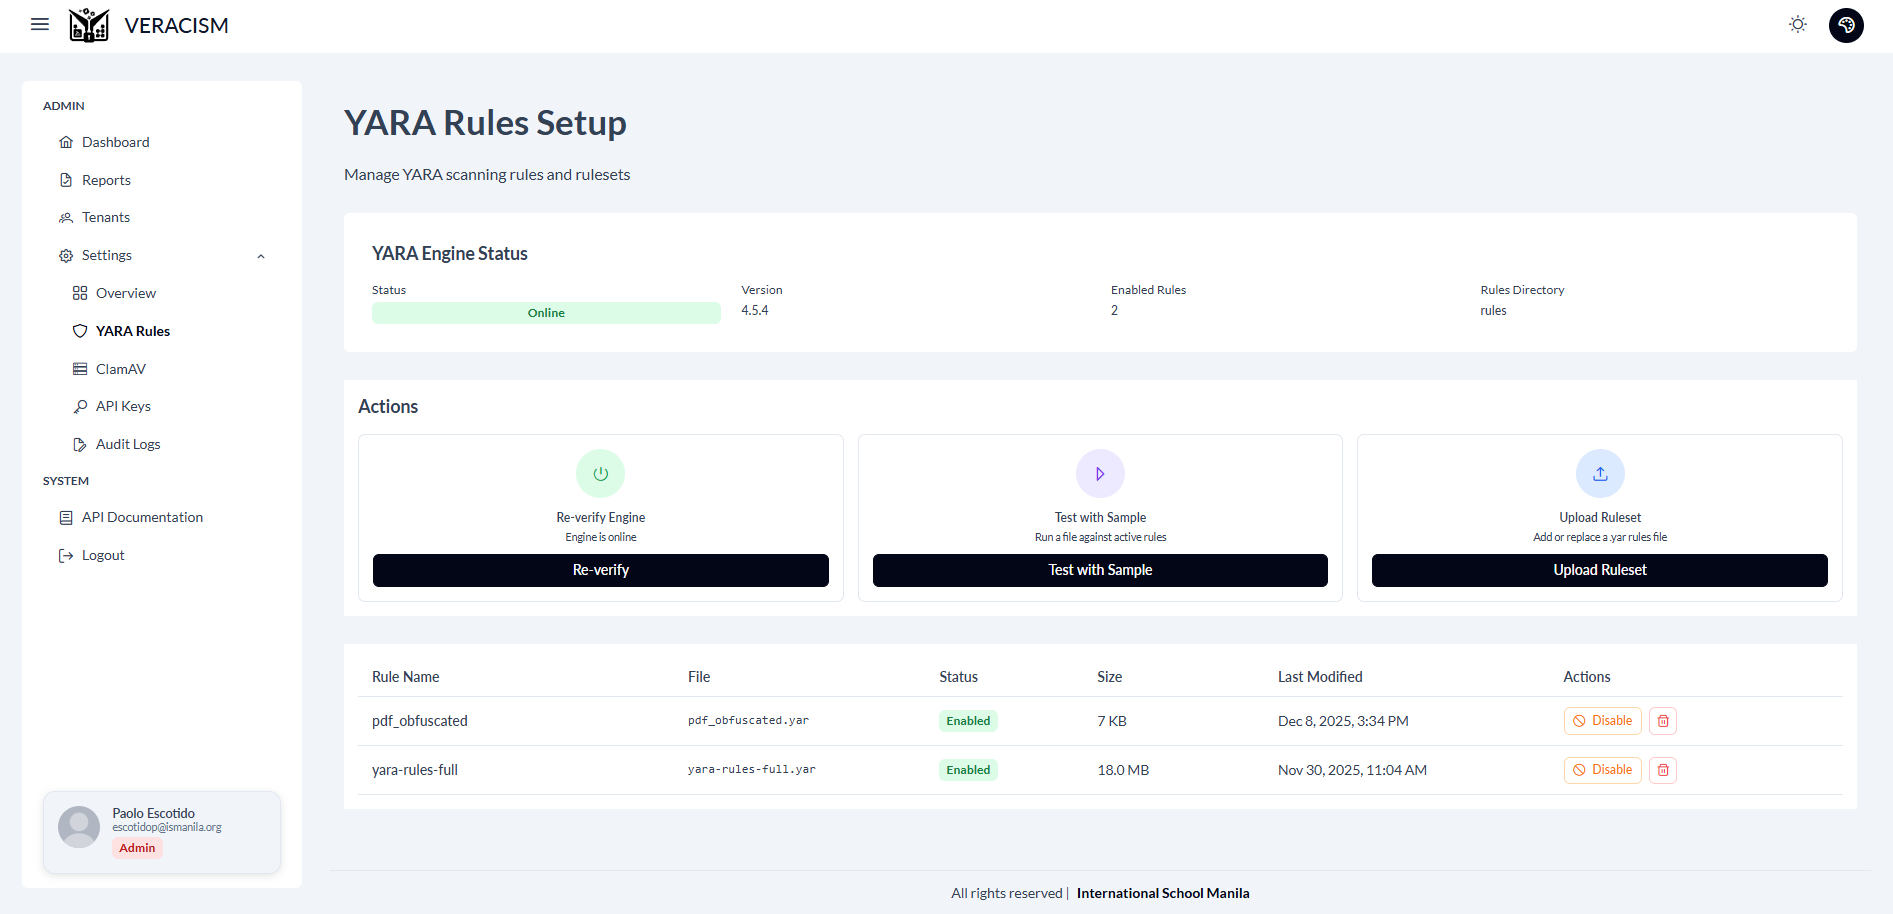
\includegraphics[height=0.35\textheight,keepaspectratio]{Texfiles/images/System Design/AdminYara.PNG}
        \caption{Admin - Yara Rules Setup}
        \label{fig:admin-yara-rules}
\end{figure}

    YARA Rules Setup page lets admins configure, enable or disable, test, and upload YARA rulesets for malware, ransomware, suspicious scripts, and custom detections.

\begin{figure}[H]
        \centering
        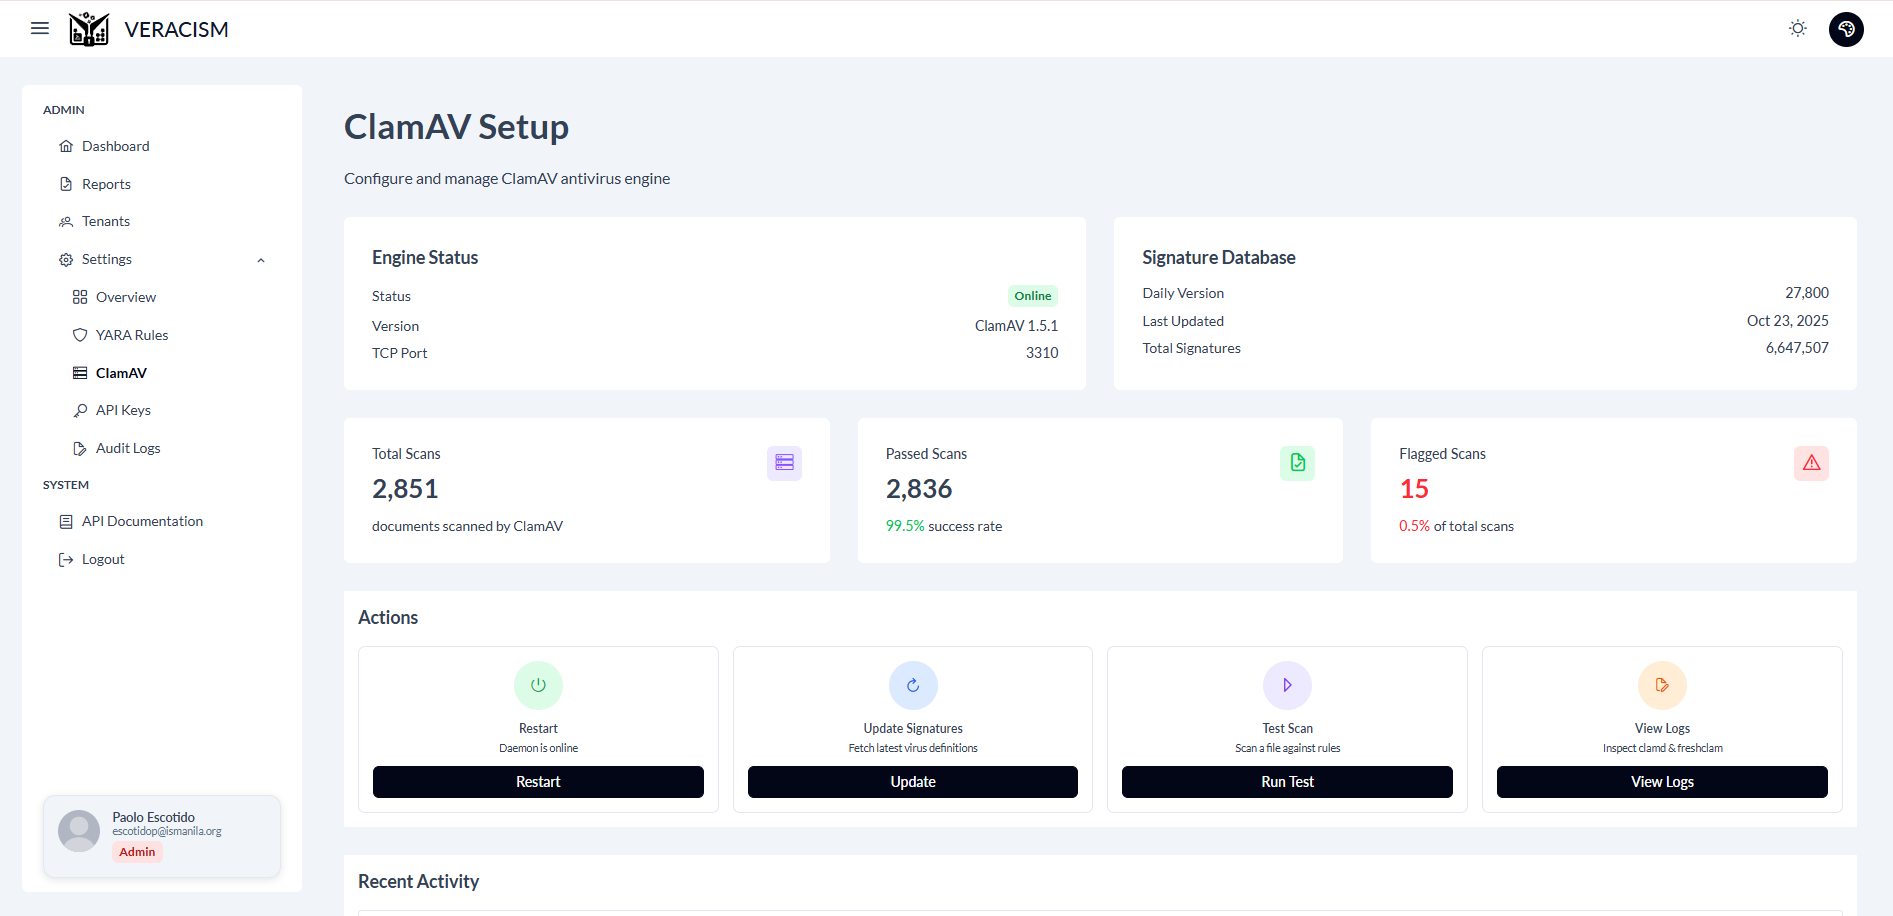
\includegraphics[height=0.35\textheight,keepaspectratio]{Texfiles/images/System Design/AdminClamAV.PNG}
        \caption{Admin - ClamAV Setup}
        \label{fig:admin-clamav}
\end{figure}

    The ClamAV Setup page lets admins monitor the antivirus engine, manage and schedule signature updates, run test scans, and review recent scan activity and statistics.

\begin{figure}[H]
        \centering
        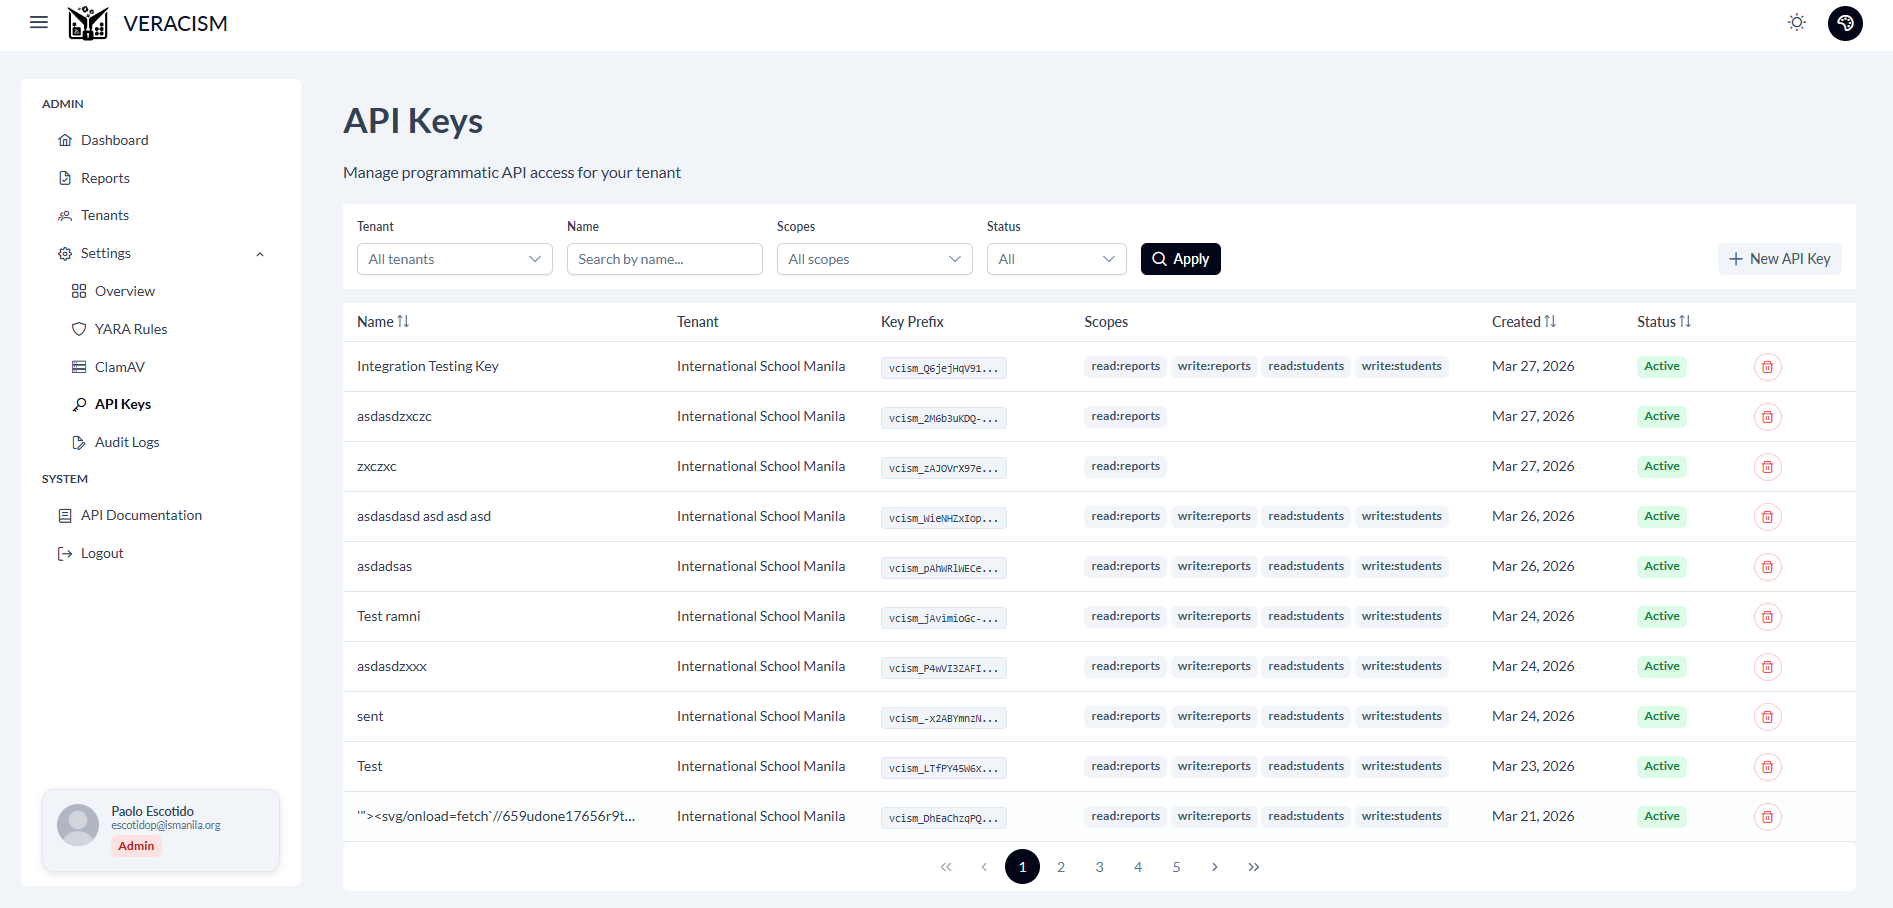
\includegraphics[height=0.35\textheight,keepaspectratio]{Texfiles/images/System Design/AdminAPIKeys.PNG}
        \caption{Admin - API Keys}
        \label{fig:admin-apikeys}
\end{figure}

    The API Keys page allows admins to manage API keys across all registered tenants. It lets them view, create, and monitor tenant API keys.

\begin{figure}[H]
        \centering
        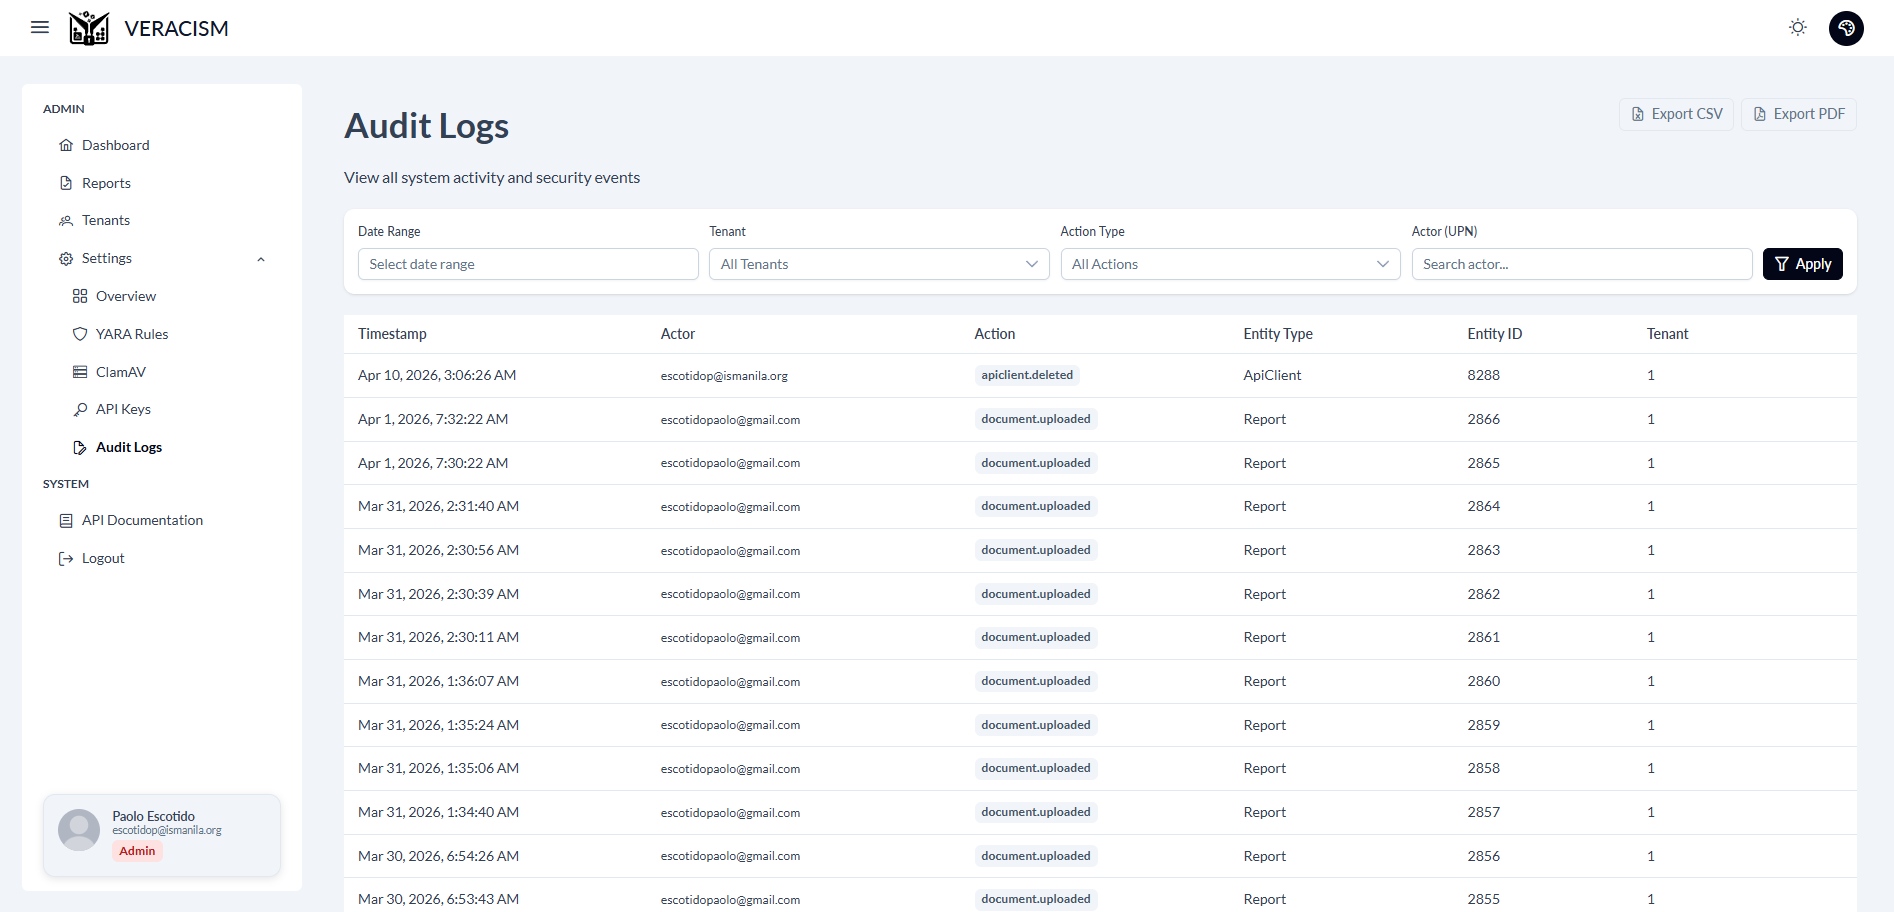
\includegraphics[height=0.35\textheight,keepaspectratio]{Texfiles/images/System Design/AdminAuditLogs.PNG}
        \caption{Admin - Audit Logs}
        \label{fig:admin-auditlogs}
\end{figure}

    The Audit Logs page lets admins review system activity and security events across all tenants. It helps track actions, actors, and affected records for monitoring and investigation.

\begin{figure}[H]
        \centering
        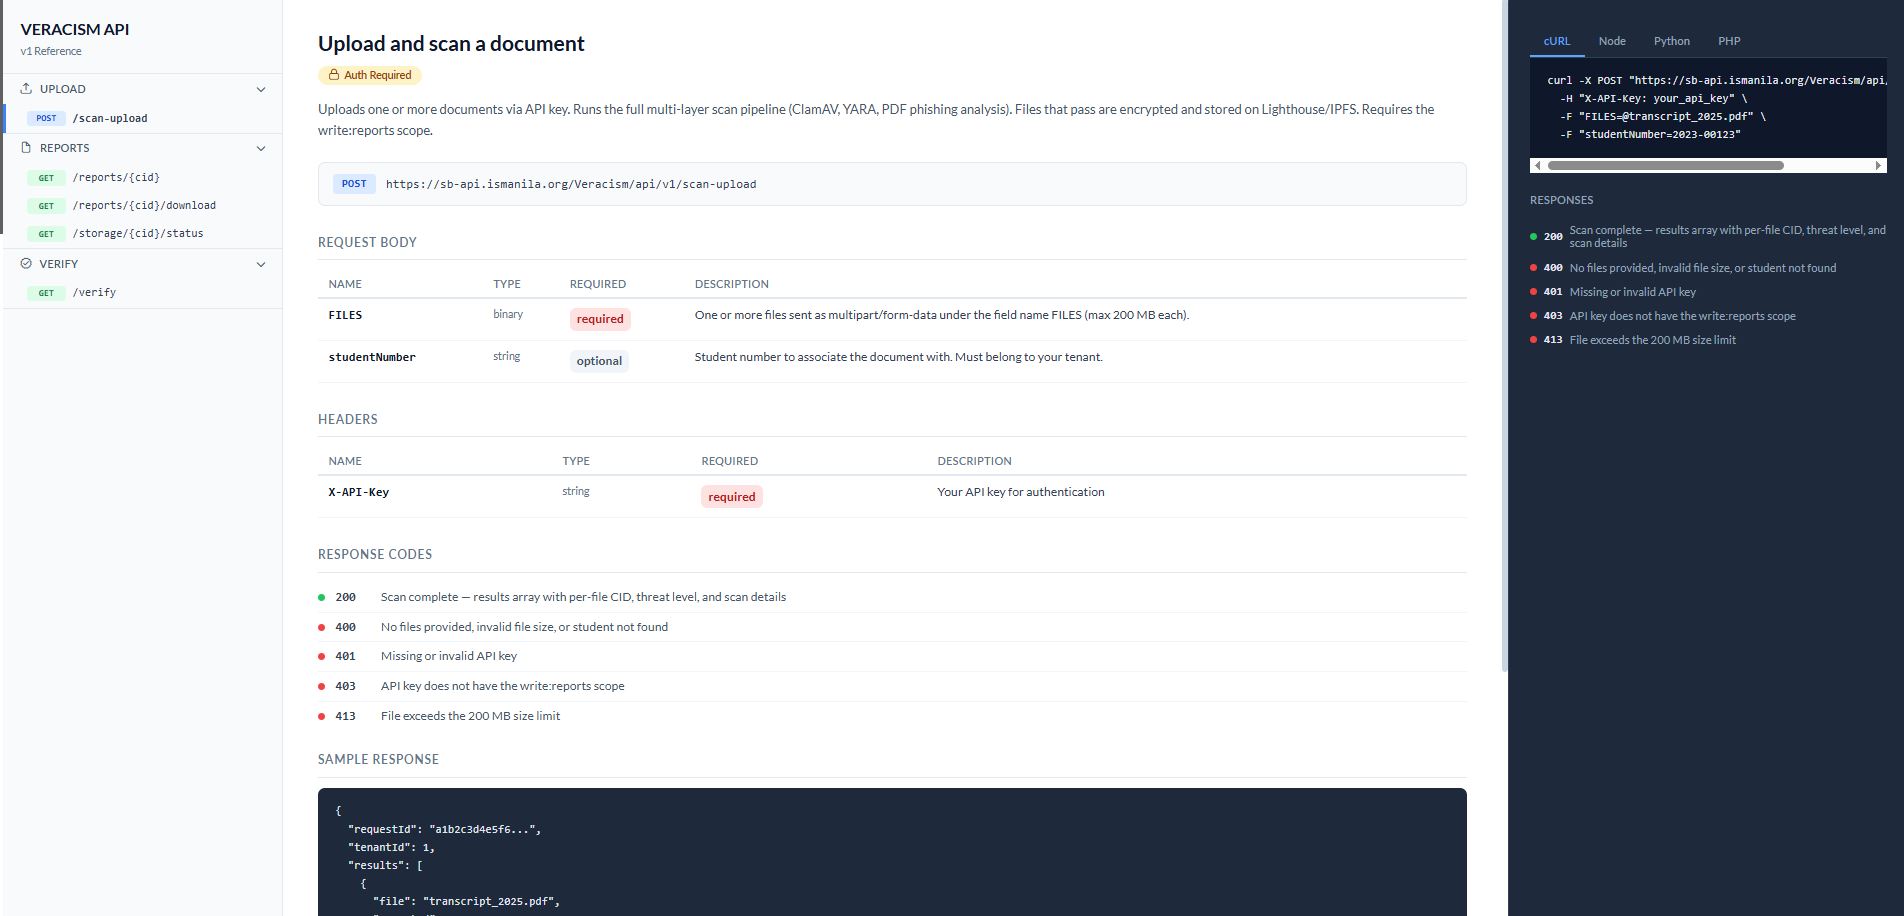
\includegraphics[height=0.35\textheight,keepaspectratio]{Texfiles/images/System Design/APIDocumentation.PNG}
        \caption{API Documentation}
        \label{fig:api-documentation}
\end{figure}

    The API Documentation page lets anyone view Veracism’s REST API base URL, key features, authentication with API keys, available endpoints, rate limits, and error codes so developers can integrate file scanning and verification into their existing systems.


\begin{figure}[H]
        \centering
        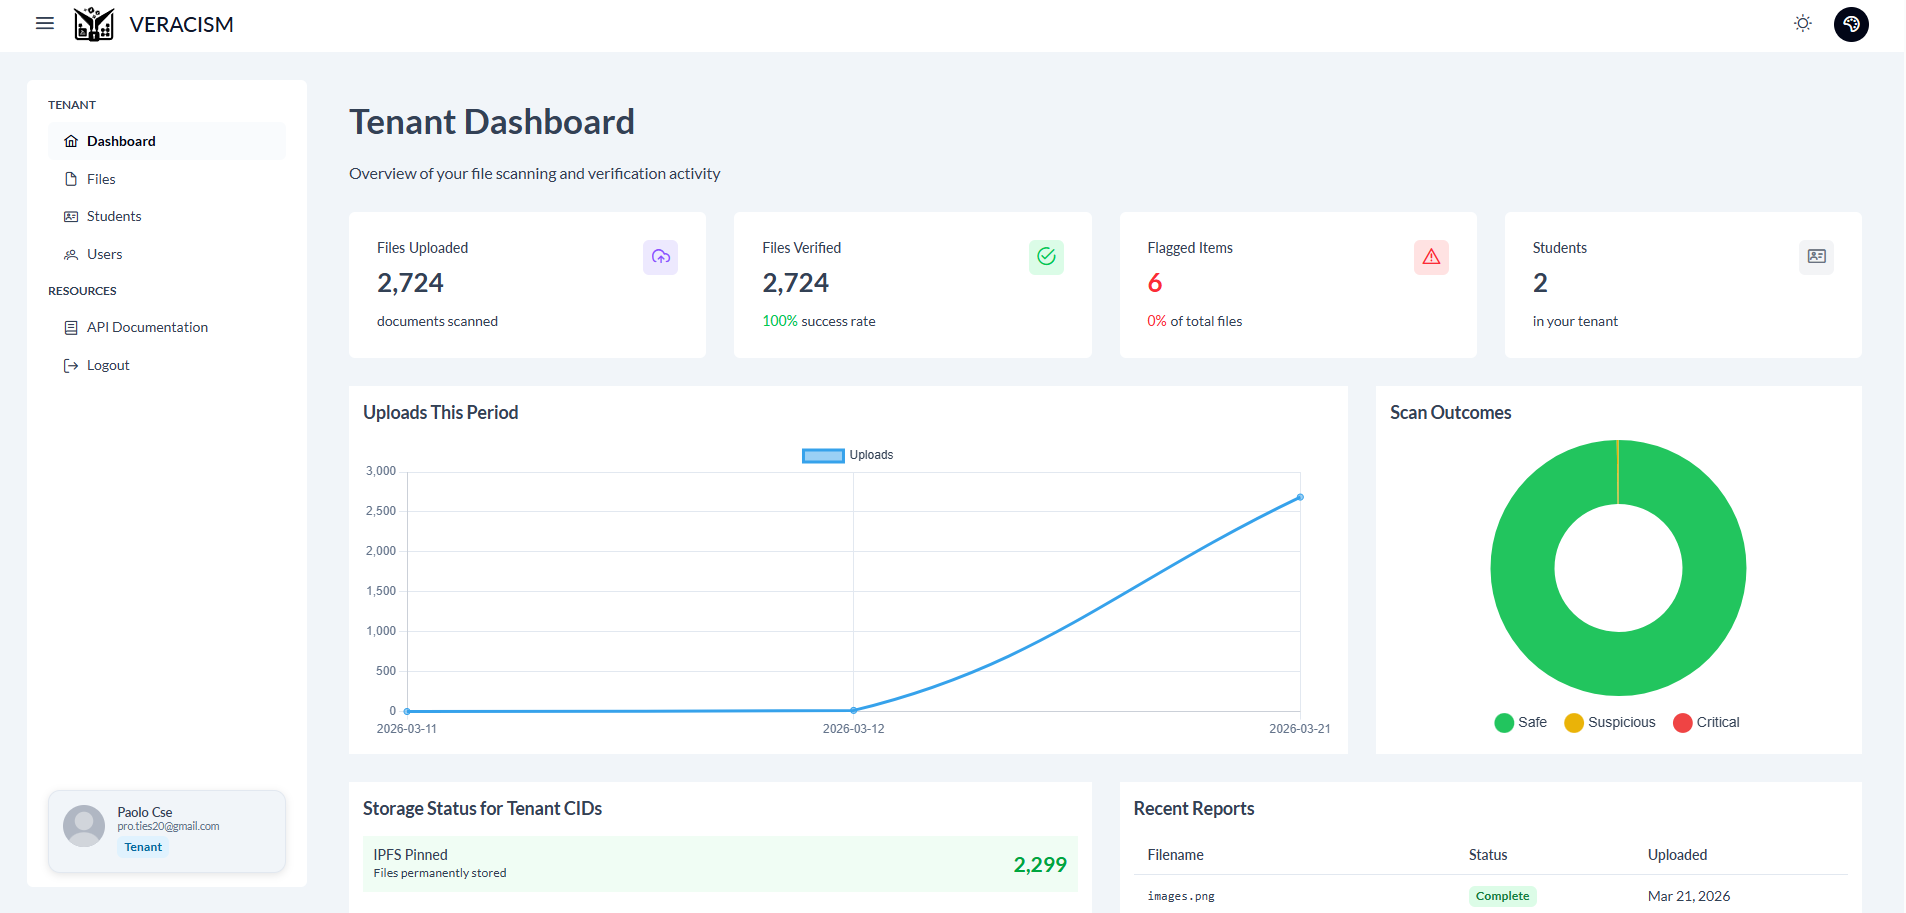
\includegraphics[height=0.35\textheight,keepaspectratio]{Texfiles/images/System Design/TenantsDashboard.PNG}
        \caption{Tenants - Dashboard}
        \label{fig:tenants-dashboard}
\end{figure}

    After tenants successfully logging into the system, the tenant is redirected to this dashboard showing their organization’s file uploads, verification success, flagged items, storage usage, upload trends, and scan outcomes. 

\begin{figure}[H]
        \centering
        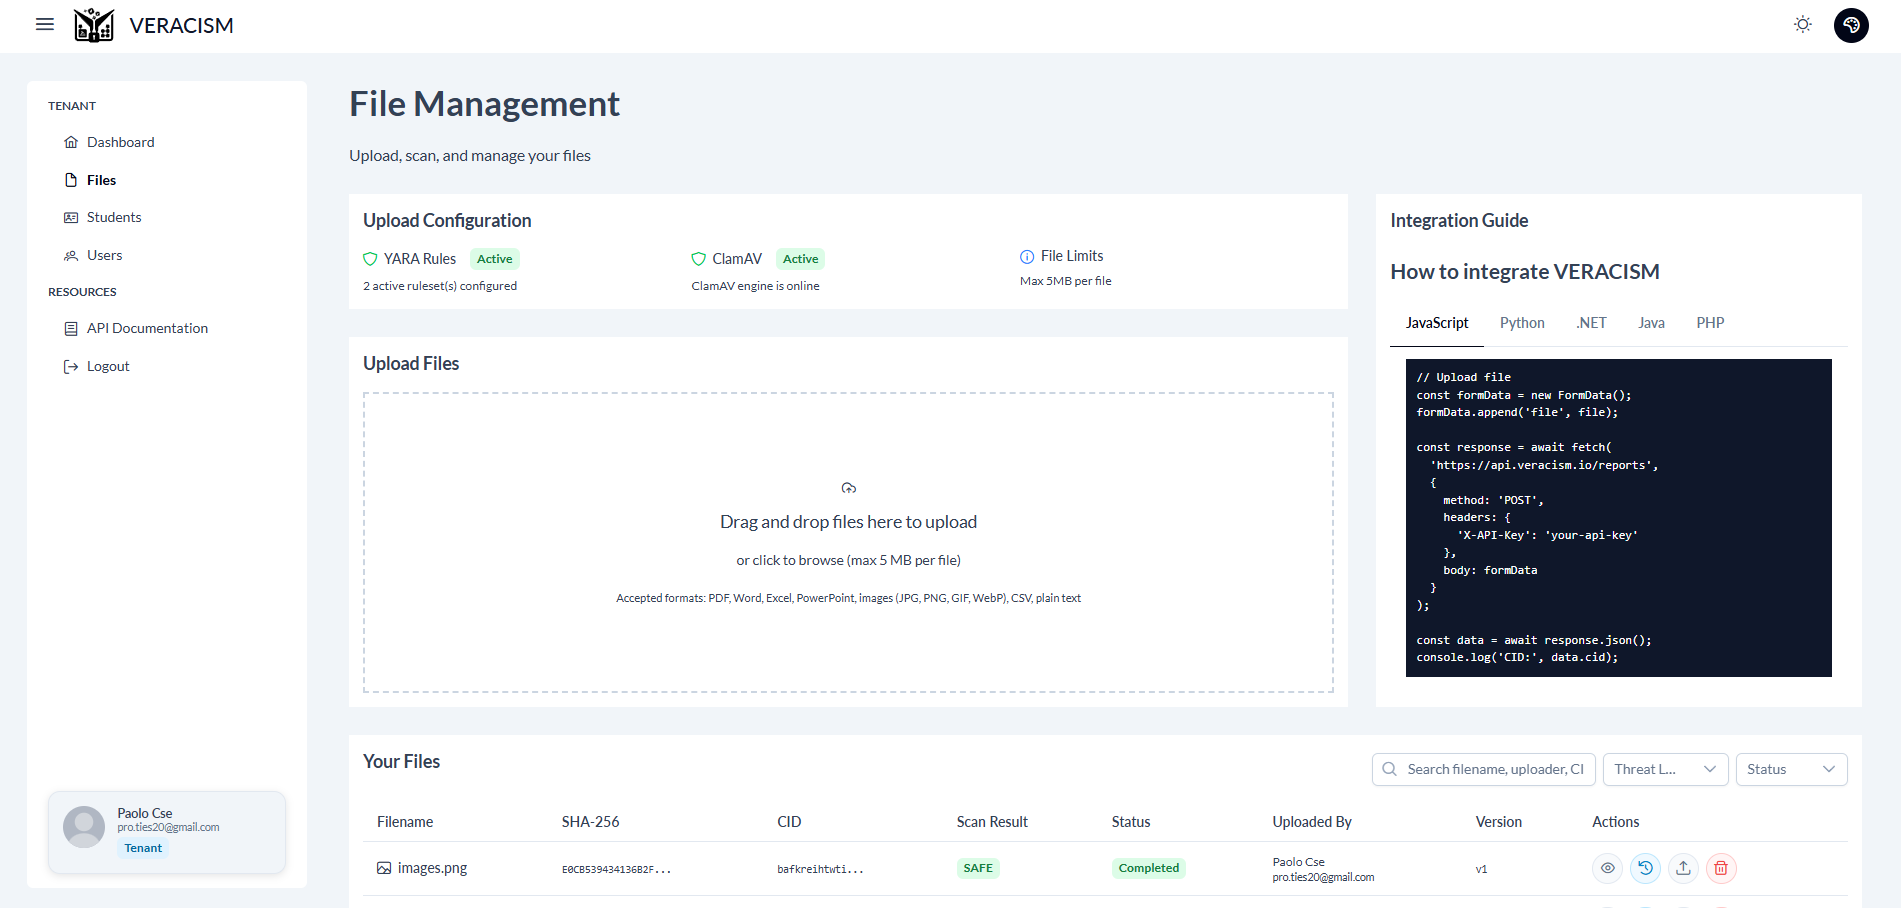
\includegraphics[height=0.35\textheight,keepaspectratio]{Texfiles/images/System Design/TenantsFileManagement.PNG}
        \caption{Tenants - File Management}
        \label{fig:tenants-filemanagement}
\end{figure}

    File management page lets tenants upload and manage their documents (view hashes, CIDs, scan results, and actions) while in the right panel, Integration Guide provides code examples showing how to call the Veracism API directly from their existing website or system.

\begin{figure}[H]
        \centering
        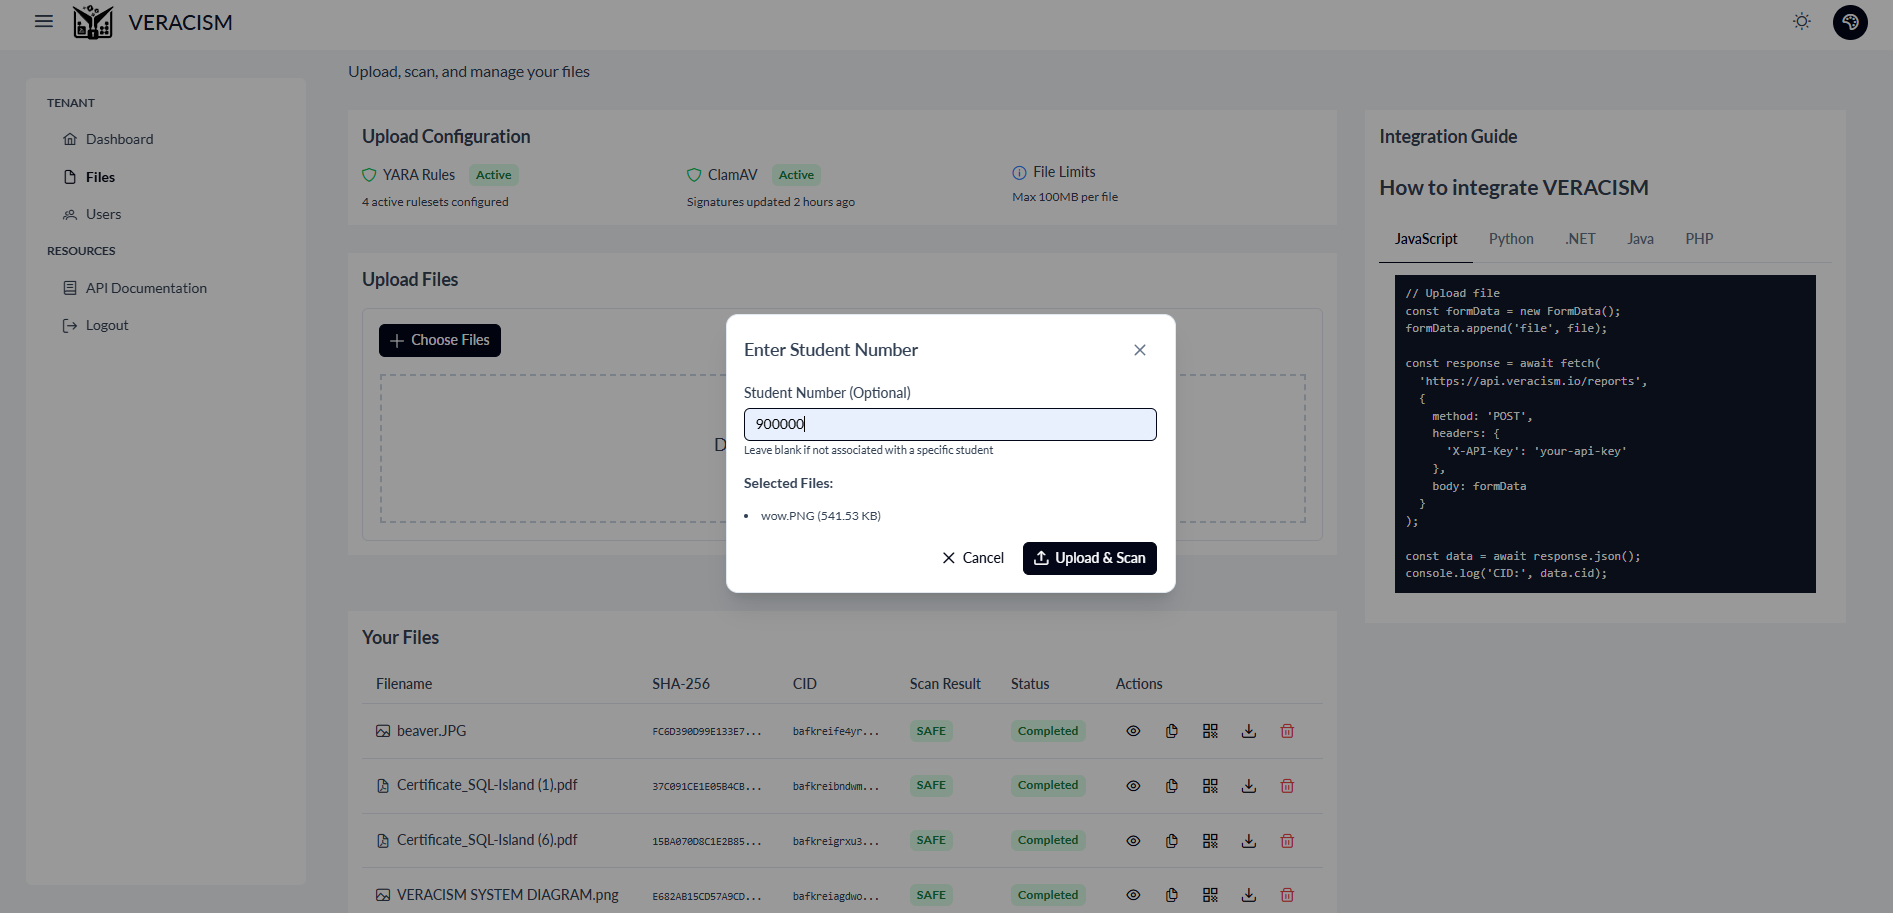
\includegraphics[height=0.35\textheight,keepaspectratio]{Texfiles/images/System Design/TenantsFileUpload.png}
        \caption{Tenants - File upload Process}
        \label{fig:tenants-file-upload}
\end{figure}

    On this upload step, tenants choose one or more files from their device and can optionally link each upload to a specific student number for easier tracking. Once submitted, the files are first scanned by the Veracism endpoint for malware, then encrypted inside Veracism using platform-managed keys. Only if a file is confirmed clean is its encrypted form written to Lighthouse storage, while its metadata (filename, size, owner, student tag), cryptographic SHA-256 hash, scan verdict, and detailed audit logs (who uploaded the file and when) are recorded in the database for future verification, traceability, and compliance reporting.

\begin{figure}[H]
        \centering
        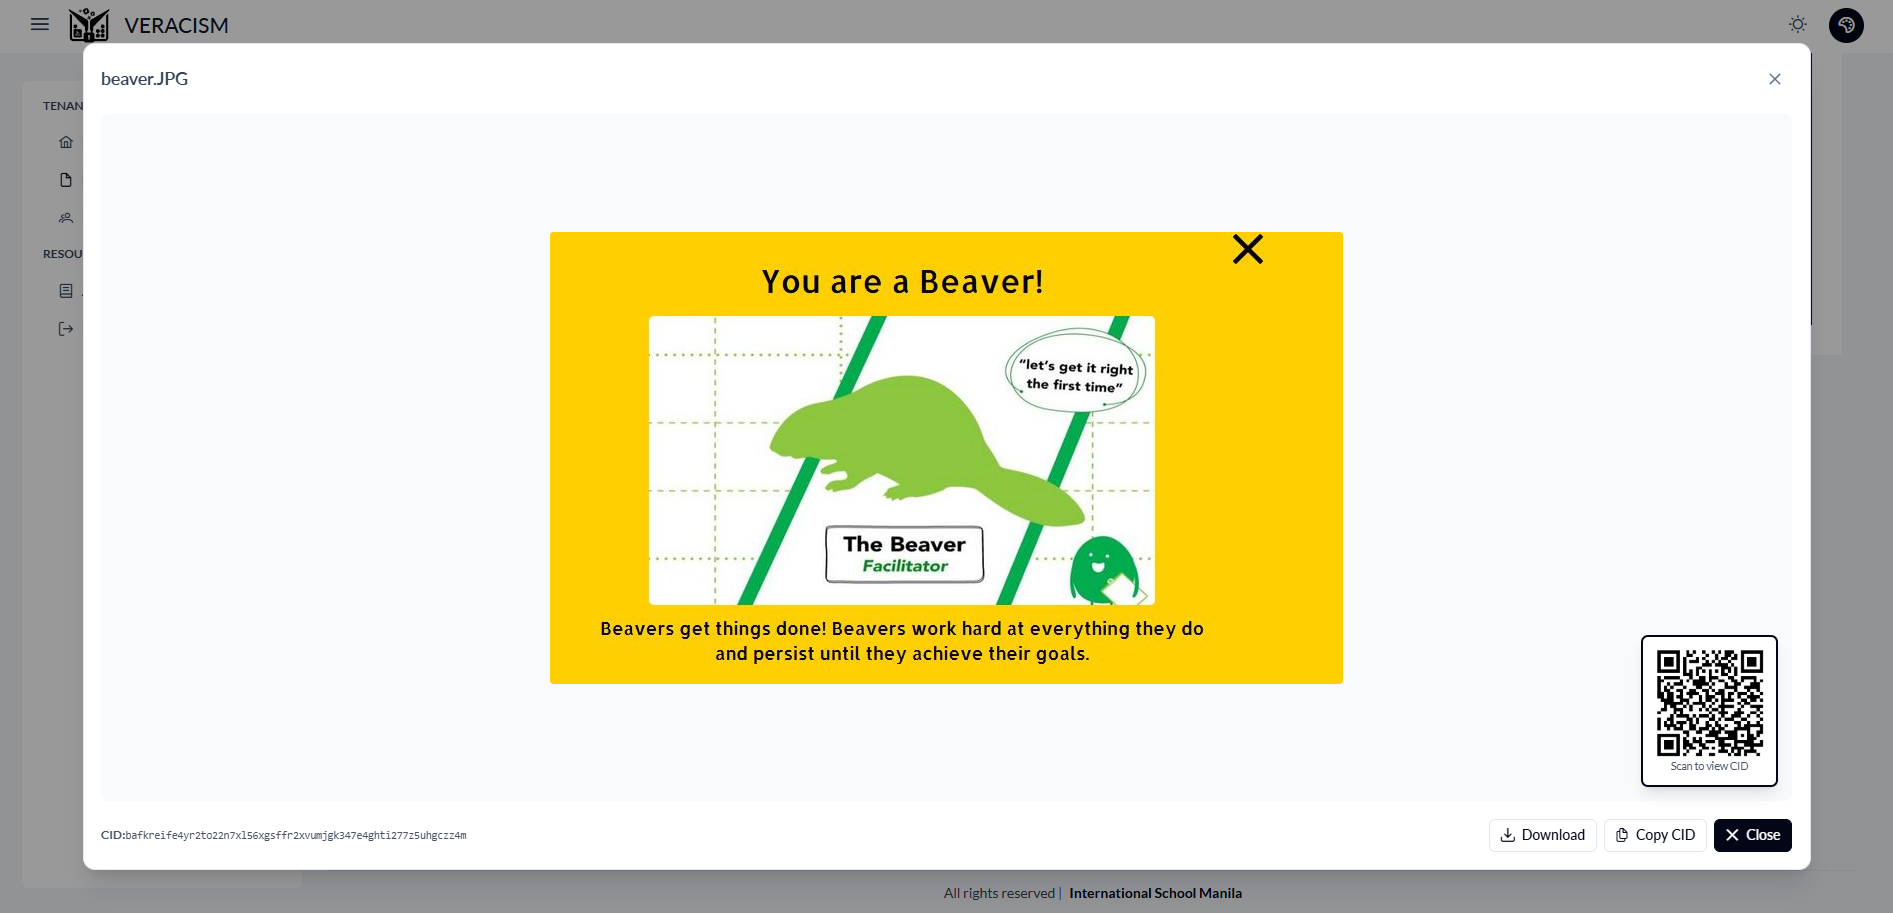
\includegraphics[height=0.35\textheight,keepaspectratio]{Texfiles/images/System Design/TenantsFileViewer.png}
        \caption{Tenants - File Viewer}
        \label{fig:tenants-file-viewer}
\end{figure}

    When a tenant chooses View on a specific file, Veracism does not stream the raw object directly from Lighthouse. Instead, the application first retrieves the encrypted blob from Lighthouse storage using a secure, signed request generated on the server. The blob is then decrypted inside Veracism using internal encryption keys that are never exposed to the tenant, Lighthouse, or any third party. Only after a successful decryption does the app render the file in a read-only viewer and show its CID, with options to download or copy the CID/QR.

    Every object stored in Lighthouse is encrypted at rest with Veracism-managed keys, anyone who obtains the direct Lighthouse URL still sees only ciphertext and cannot reconstruct the original file. This completes an end-to-end protection flow in which:


\begin{enumerate}
    \item Files are encrypted before being written to Lighthouse.
    \item Encrypted objects are stored and replicated by Lighthouse without access to plaintext.
    \item Only the Veracism backend can decrypt and serve a temporary, view-only version to authenticated tenants based on their access rights.
\end{enumerate}


\begin{figure}[H]
        \centering
        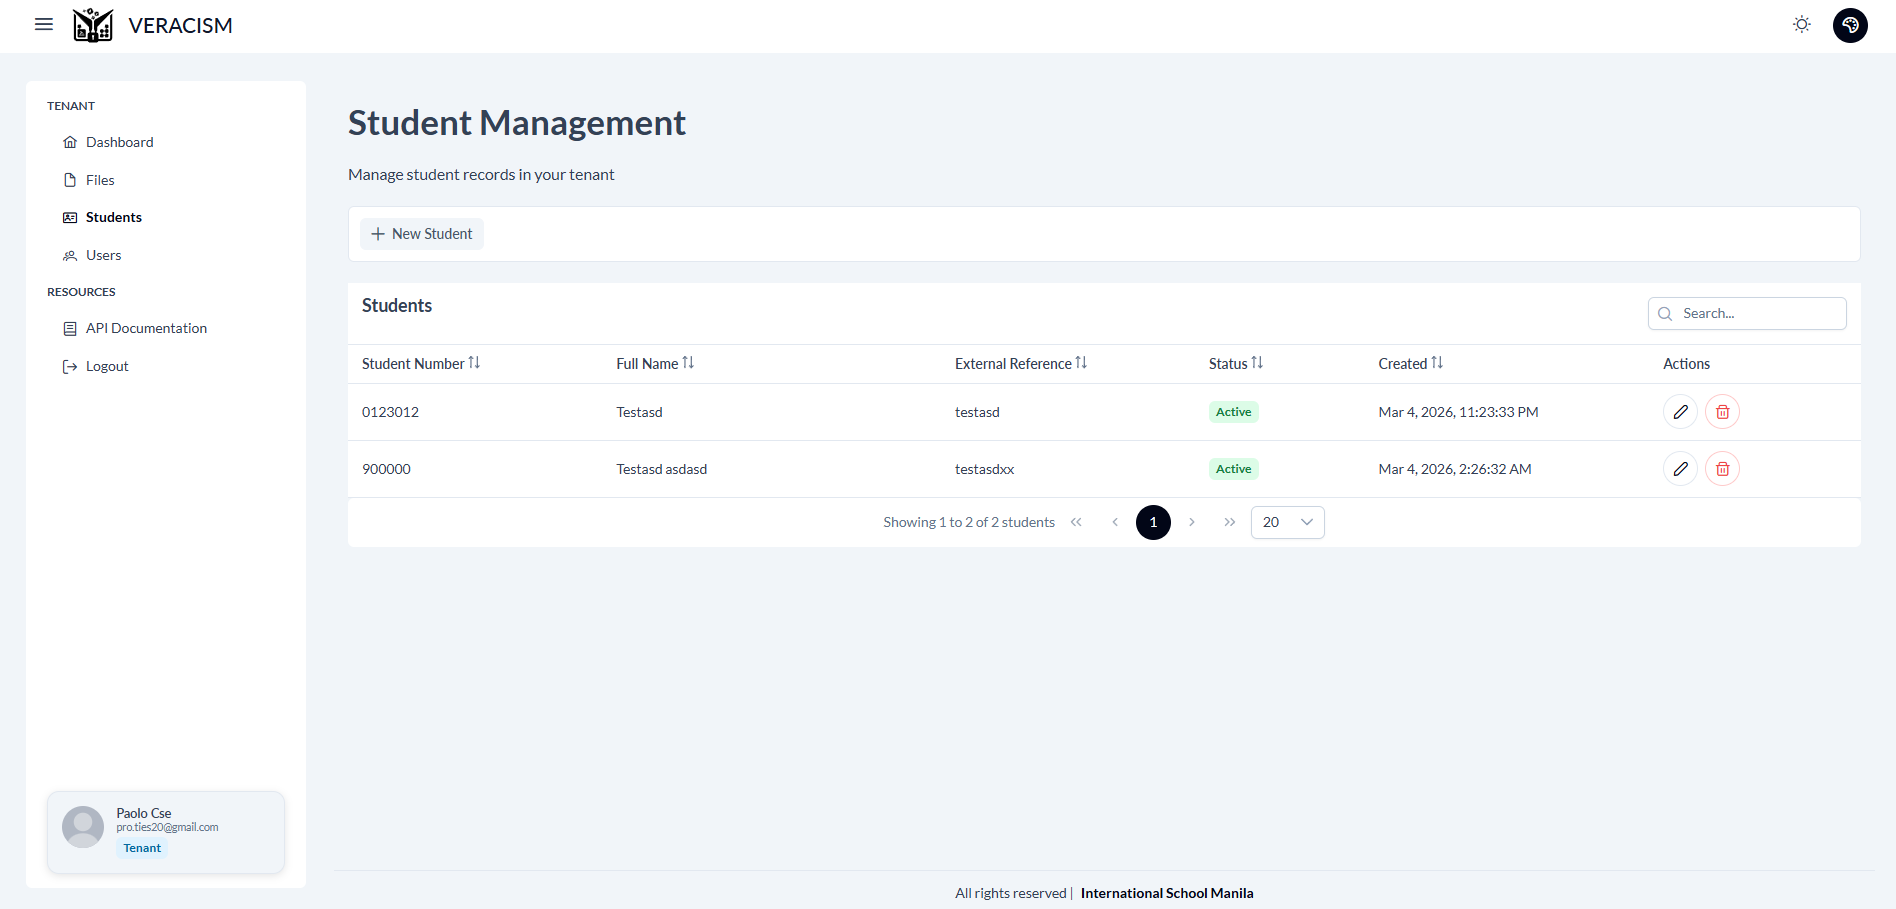
\includegraphics[height=0.35\textheight,keepaspectratio]{Texfiles/images/System Design/TenantsStudentsManagement.PNG}
        \caption{Tenants - Student Management}
        \label{fig:tenants-student-management}
\end{figure}

    The Student Management page lets tenant users manage student records within their tenant. It allows them to add, view, search, and update student information.

\begin{figure}[H]
        \centering
        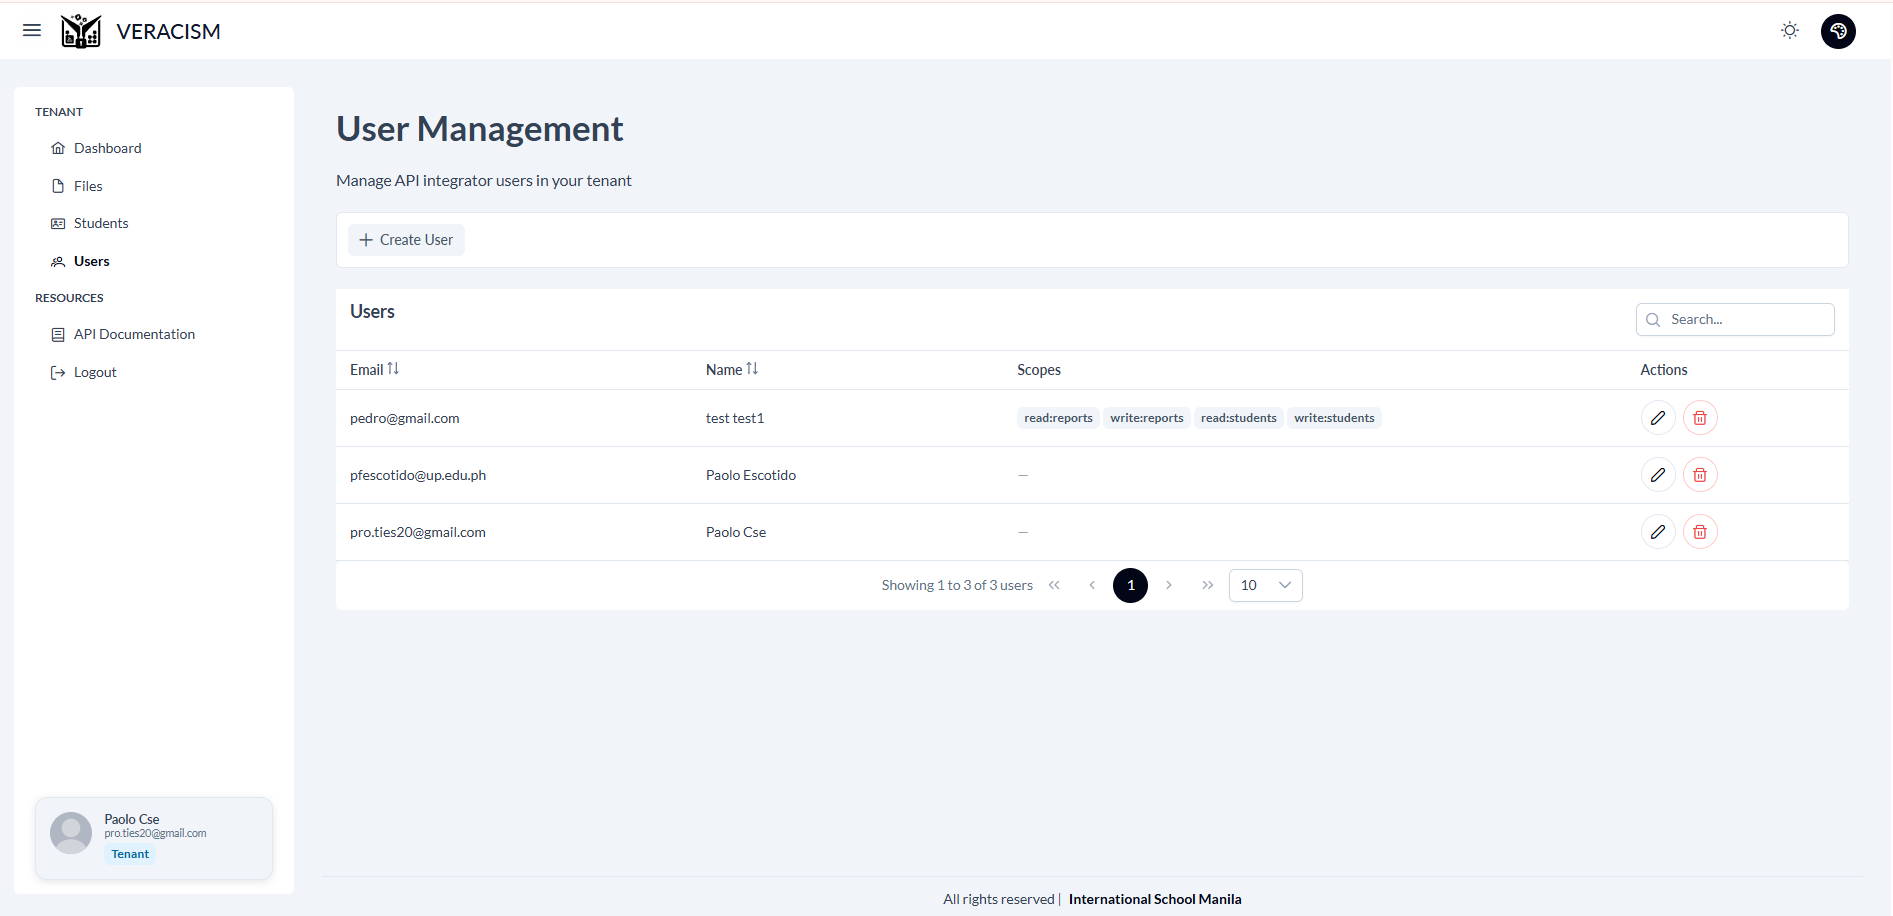
\includegraphics[height=0.35\textheight,keepaspectratio]{Texfiles/images/System Design/TenantsUserManagement.PNG}
        \caption{Tenants - User Management}
        \label{fig:tenants-user-management}
\end{figure}

    Tenant User Management page lets each organization fully control who can access and integrate with Veracism under their tenant. From a single view, tenant admins can invite new integrators by email, assign or change roles (such as Admin or Member), update user details, and enable or disable accounts without losing their history. The table shows current status and last login time for every user, helping admins monitor who is actively using the system. For technical users and integrations, admins can also generate and rotate tenant-scoped API keys per account, so every API call is tied to a specific user for fine-grained access control, easier revocation, and clear auditability.
\clearpage